% Options for packages loaded elsewhere
\PassOptionsToPackage{unicode}{hyperref}
\PassOptionsToPackage{hyphens}{url}
%
\documentclass[
]{article}
\usepackage{amsmath,amssymb}
\usepackage{lmodern}
\usepackage{ifxetex,ifluatex}
\ifnum 0\ifxetex 1\fi\ifluatex 1\fi=0 % if pdftex
  \usepackage[T1]{fontenc}
  \usepackage[utf8]{inputenc}
  \usepackage{textcomp} % provide euro and other symbols
\else % if luatex or xetex
  \usepackage{unicode-math}
  \defaultfontfeatures{Scale=MatchLowercase}
  \defaultfontfeatures[\rmfamily]{Ligatures=TeX,Scale=1}
\fi
% Use upquote if available, for straight quotes in verbatim environments
\IfFileExists{upquote.sty}{\usepackage{upquote}}{}
\IfFileExists{microtype.sty}{% use microtype if available
  \usepackage[]{microtype}
  \UseMicrotypeSet[protrusion]{basicmath} % disable protrusion for tt fonts
}{}
\makeatletter
\@ifundefined{KOMAClassName}{% if non-KOMA class
  \IfFileExists{parskip.sty}{%
    \usepackage{parskip}
  }{% else
    \setlength{\parindent}{0pt}
    \setlength{\parskip}{6pt plus 2pt minus 1pt}}
}{% if KOMA class
  \KOMAoptions{parskip=half}}
\makeatother
\usepackage{xcolor}
\IfFileExists{xurl.sty}{\usepackage{xurl}}{} % add URL line breaks if available
\IfFileExists{bookmark.sty}{\usepackage{bookmark}}{\usepackage{hyperref}}
\hypersetup{
  pdftitle={Lab1},
  pdfauthor={Andrew Laws},
  hidelinks,
  pdfcreator={LaTeX via pandoc}}
\urlstyle{same} % disable monospaced font for URLs
\usepackage[margin=1in]{geometry}
\usepackage{color}
\usepackage{fancyvrb}
\newcommand{\VerbBar}{|}
\newcommand{\VERB}{\Verb[commandchars=\\\{\}]}
\DefineVerbatimEnvironment{Highlighting}{Verbatim}{commandchars=\\\{\}}
% Add ',fontsize=\small' for more characters per line
\usepackage{framed}
\definecolor{shadecolor}{RGB}{248,248,248}
\newenvironment{Shaded}{\begin{snugshade}}{\end{snugshade}}
\newcommand{\AlertTok}[1]{\textcolor[rgb]{0.94,0.16,0.16}{#1}}
\newcommand{\AnnotationTok}[1]{\textcolor[rgb]{0.56,0.35,0.01}{\textbf{\textit{#1}}}}
\newcommand{\AttributeTok}[1]{\textcolor[rgb]{0.77,0.63,0.00}{#1}}
\newcommand{\BaseNTok}[1]{\textcolor[rgb]{0.00,0.00,0.81}{#1}}
\newcommand{\BuiltInTok}[1]{#1}
\newcommand{\CharTok}[1]{\textcolor[rgb]{0.31,0.60,0.02}{#1}}
\newcommand{\CommentTok}[1]{\textcolor[rgb]{0.56,0.35,0.01}{\textit{#1}}}
\newcommand{\CommentVarTok}[1]{\textcolor[rgb]{0.56,0.35,0.01}{\textbf{\textit{#1}}}}
\newcommand{\ConstantTok}[1]{\textcolor[rgb]{0.00,0.00,0.00}{#1}}
\newcommand{\ControlFlowTok}[1]{\textcolor[rgb]{0.13,0.29,0.53}{\textbf{#1}}}
\newcommand{\DataTypeTok}[1]{\textcolor[rgb]{0.13,0.29,0.53}{#1}}
\newcommand{\DecValTok}[1]{\textcolor[rgb]{0.00,0.00,0.81}{#1}}
\newcommand{\DocumentationTok}[1]{\textcolor[rgb]{0.56,0.35,0.01}{\textbf{\textit{#1}}}}
\newcommand{\ErrorTok}[1]{\textcolor[rgb]{0.64,0.00,0.00}{\textbf{#1}}}
\newcommand{\ExtensionTok}[1]{#1}
\newcommand{\FloatTok}[1]{\textcolor[rgb]{0.00,0.00,0.81}{#1}}
\newcommand{\FunctionTok}[1]{\textcolor[rgb]{0.00,0.00,0.00}{#1}}
\newcommand{\ImportTok}[1]{#1}
\newcommand{\InformationTok}[1]{\textcolor[rgb]{0.56,0.35,0.01}{\textbf{\textit{#1}}}}
\newcommand{\KeywordTok}[1]{\textcolor[rgb]{0.13,0.29,0.53}{\textbf{#1}}}
\newcommand{\NormalTok}[1]{#1}
\newcommand{\OperatorTok}[1]{\textcolor[rgb]{0.81,0.36,0.00}{\textbf{#1}}}
\newcommand{\OtherTok}[1]{\textcolor[rgb]{0.56,0.35,0.01}{#1}}
\newcommand{\PreprocessorTok}[1]{\textcolor[rgb]{0.56,0.35,0.01}{\textit{#1}}}
\newcommand{\RegionMarkerTok}[1]{#1}
\newcommand{\SpecialCharTok}[1]{\textcolor[rgb]{0.00,0.00,0.00}{#1}}
\newcommand{\SpecialStringTok}[1]{\textcolor[rgb]{0.31,0.60,0.02}{#1}}
\newcommand{\StringTok}[1]{\textcolor[rgb]{0.31,0.60,0.02}{#1}}
\newcommand{\VariableTok}[1]{\textcolor[rgb]{0.00,0.00,0.00}{#1}}
\newcommand{\VerbatimStringTok}[1]{\textcolor[rgb]{0.31,0.60,0.02}{#1}}
\newcommand{\WarningTok}[1]{\textcolor[rgb]{0.56,0.35,0.01}{\textbf{\textit{#1}}}}
\usepackage{graphicx}
\makeatletter
\def\maxwidth{\ifdim\Gin@nat@width>\linewidth\linewidth\else\Gin@nat@width\fi}
\def\maxheight{\ifdim\Gin@nat@height>\textheight\textheight\else\Gin@nat@height\fi}
\makeatother
% Scale images if necessary, so that they will not overflow the page
% margins by default, and it is still possible to overwrite the defaults
% using explicit options in \includegraphics[width, height, ...]{}
\setkeys{Gin}{width=\maxwidth,height=\maxheight,keepaspectratio}
% Set default figure placement to htbp
\makeatletter
\def\fps@figure{htbp}
\makeatother
\setlength{\emergencystretch}{3em} % prevent overfull lines
\providecommand{\tightlist}{%
  \setlength{\itemsep}{0pt}\setlength{\parskip}{0pt}}
\setcounter{secnumdepth}{-\maxdimen} % remove section numbering
\ifluatex
  \usepackage{selnolig}  % disable illegal ligatures
\fi

\title{Lab1}
\author{Andrew Laws}
\date{9/10/2021}

\begin{document}
\maketitle

\hypertarget{task-1-basic-data-manipulation}{%
\section{Task 1: Basic data
manipulation}\label{task-1-basic-data-manipulation}}

\hypertarget{section}{%
\subsubsection{1.1}\label{section}}

\begin{Shaded}
\begin{Highlighting}[]
\CommentTok{\#create new df}
\NormalTok{task1}\FloatTok{.1} \OtherTok{\textless{}{-}}\NormalTok{ d.counties }\SpecialCharTok{\%\textgreater{}\%} \FunctionTok{group\_by}\NormalTok{(STATEFP10) }\SpecialCharTok{\%\textgreater{}\%} \CommentTok{\#group variables by state and mutate column that holds state area}
  \FunctionTok{mutate}\NormalTok{(}\AttributeTok{stateArea =} \FunctionTok{sum}\NormalTok{(ALAND10 }\SpecialCharTok{+}\NormalTok{ AWATER10)) }\SpecialCharTok{\%\textgreater{}\%} \CommentTok{\#mutate column that divides land area by state area}
  \FunctionTok{ungroup}\NormalTok{(.) }\SpecialCharTok{\%\textgreater{}\%} 
  \FunctionTok{mutate}\NormalTok{(}\AttributeTok{perLandAreaState =}\NormalTok{ ALAND10}\SpecialCharTok{/}\NormalTok{stateArea }\SpecialCharTok{*} \DecValTok{100}\NormalTok{) }\CommentTok{\#create percentage variable by dividing land by state area and multiplying by 100}

\FunctionTok{glimpse}\NormalTok{(task1}\FloatTok{.1}\SpecialCharTok{$}\NormalTok{perLandAreaState)}
\end{Highlighting}
\end{Shaded}

\begin{verbatim}
##  num [1:207] 0.0342 0.0502 0.0224 0.0208 2.2555 ...
\end{verbatim}

\hypertarget{section-1}{%
\subsubsection{1.2}\label{section-1}}

\begin{Shaded}
\begin{Highlighting}[]
\CommentTok{\#group by state, find max of awater10/state area using slice}
\NormalTok{task1}\FloatTok{.2} \OtherTok{\textless{}{-}}\NormalTok{ task1}\FloatTok{.1} \SpecialCharTok{\%\textgreater{}\%} \FunctionTok{as\_tibble}\NormalTok{() }\SpecialCharTok{\%\textgreater{}\%} 
  \FunctionTok{group\_by}\NormalTok{(STATEFP10) }\SpecialCharTok{\%\textgreater{}\%} 
  \FunctionTok{mutate}\NormalTok{(}\AttributeTok{perWaterAreaState =}\NormalTok{ AWATER10}\SpecialCharTok{/}\NormalTok{stateArea }\SpecialCharTok{*} \DecValTok{100}\NormalTok{) }\SpecialCharTok{\%\textgreater{}\%} 
  \FunctionTok{slice}\NormalTok{(}\FunctionTok{which.max}\NormalTok{(perWaterAreaState))}

\CommentTok{\#create df with only state and county name columns}
\NormalTok{wettest\_counties }\OtherTok{\textless{}{-}}\NormalTok{ task1}\FloatTok{.2} \SpecialCharTok{\%\textgreater{}\%} \FunctionTok{ungroup}\NormalTok{() }\SpecialCharTok{\%\textgreater{}\%} 
\NormalTok{  dplyr}\SpecialCharTok{::}\FunctionTok{select}\NormalTok{(STATEFP10, NAMELSAD10)}
\NormalTok{wettest\_counties}
\end{Highlighting}
\end{Shaded}

\begin{verbatim}
## # A tibble: 7 x 2
##   STATEFP10 NAMELSAD10          
##   <chr>     <chr>               
## 1 10        Sussex County       
## 2 11        District of Columbia
## 3 24        Dorchester County   
## 4 36        Cayuga County       
## 5 42        Lancaster County    
## 6 51        Accomack County     
## 7 54        Greenbrier County
\end{verbatim}

\hypertarget{section-2}{%
\subsubsection{1.3}\label{section-2}}

\begin{Shaded}
\begin{Highlighting}[]
\CommentTok{\#Use count function }
\NormalTok{task1}\FloatTok{.3} \OtherTok{\textless{}{-}}\NormalTok{ d.counties }\SpecialCharTok{\%\textgreater{}\%}\NormalTok{ as\_tibble }\SpecialCharTok{\%\textgreater{}\%} 
  \FunctionTok{count}\NormalTok{(STATEFP10)}
\NormalTok{task1}\FloatTok{.3}
\end{Highlighting}
\end{Shaded}

\begin{verbatim}
## # A tibble: 7 x 2
##   STATEFP10     n
##   <chr>     <int>
## 1 10            3
## 2 11            1
## 3 24           24
## 4 36           20
## 5 42           43
## 6 51          102
## 7 54           14
\end{verbatim}

\hypertarget{section-3}{%
\subsubsection{1.4}\label{section-3}}

\begin{Shaded}
\begin{Highlighting}[]
\CommentTok{\#use mutate function to create new column with character length}
\NormalTok{task1}\FloatTok{.4} \OtherTok{\textless{}{-}}\NormalTok{ d.stations }\SpecialCharTok{\%\textgreater{}\%} \FunctionTok{as\_tibble}\NormalTok{() }\SpecialCharTok{\%\textgreater{}\%} 
  \FunctionTok{mutate}\NormalTok{(., }\AttributeTok{stNameLen =} \FunctionTok{nchar}\NormalTok{(STATION\_NA)) }\SpecialCharTok{\%\textgreater{}\%}  
  \FunctionTok{slice}\NormalTok{(}\FunctionTok{which.min}\NormalTok{(stNameLen)) }\SpecialCharTok{\%\textgreater{}\%} \CommentTok{\#slice out the row with the min number of characters}
\NormalTok{  dplyr}\SpecialCharTok{::}\FunctionTok{select}\NormalTok{(STATION\_NA) }\CommentTok{\#retain only station name}

\NormalTok{task1}\FloatTok{.4}
\end{Highlighting}
\end{Shaded}

\begin{verbatim}
## # A tibble: 1 x 1
##   STATION_NA                
##   <chr>                     
## 1 ABRAM CREEK AT OAKMONT, WV
\end{verbatim}

\hypertarget{task-2-plotting-attribute-data}{%
\section{Task 2: Plotting attribute
data}\label{task-2-plotting-attribute-data}}

\hypertarget{section-4}{%
\subsubsection{2.1}\label{section-4}}

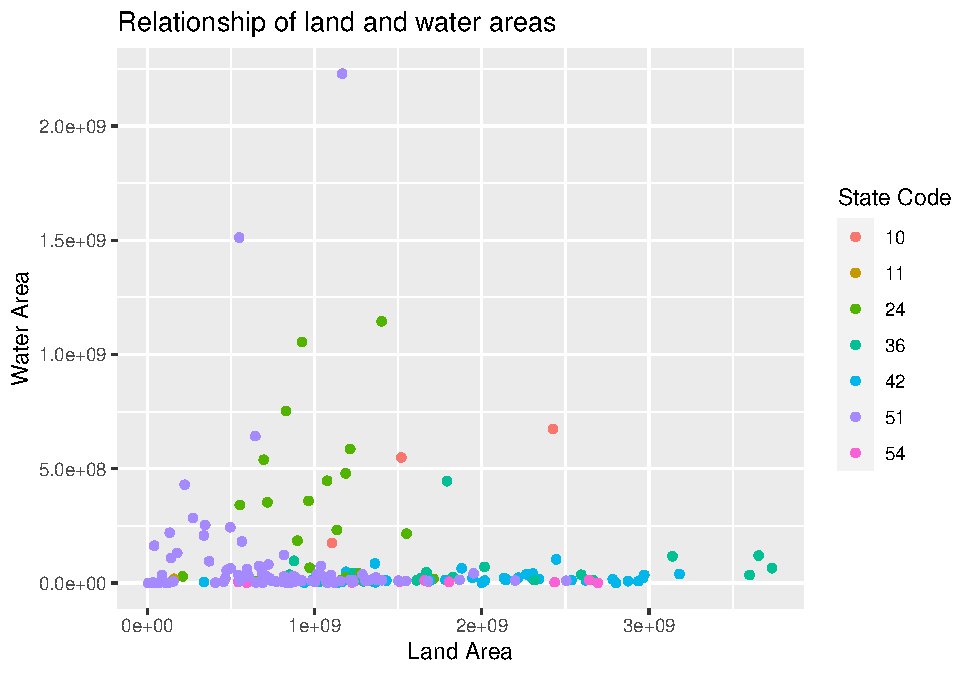
\includegraphics{Lab1_files/figure-latex/2.1-1.pdf}

\hypertarget{section-5}{%
\subsubsection{2.2}\label{section-5}}

\begin{verbatim}
## `stat_bin()` using `bins = 30`. Pick better value with `binwidth`.
\end{verbatim}

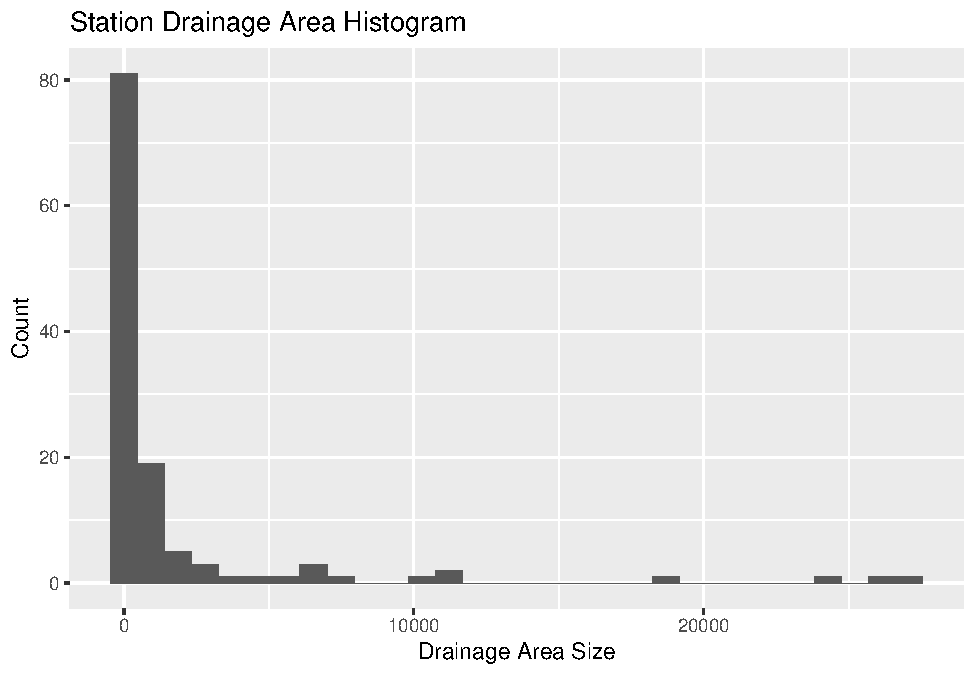
\includegraphics{Lab1_files/figure-latex/2.2-1.pdf}

\hypertarget{section-6}{%
\subsubsection{2.3}\label{section-6}}

\begin{verbatim}
## `stat_bin()` using `bins = 30`. Pick better value with `binwidth`.
\end{verbatim}

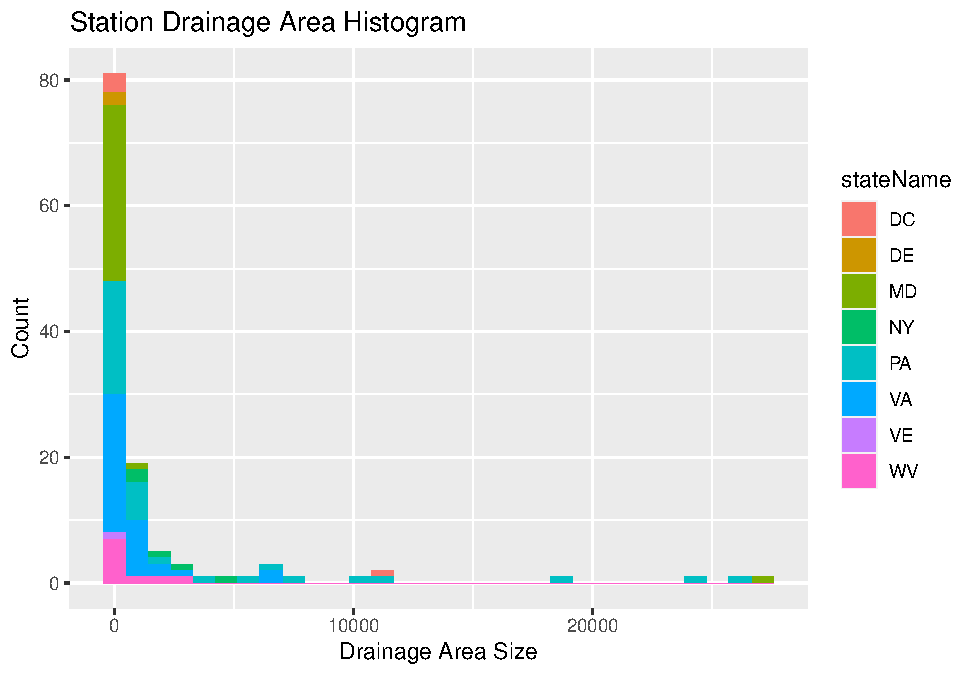
\includegraphics{Lab1_files/figure-latex/2.3-1.pdf}

\hypertarget{task-3-write-a-function}{%
\section{Task 3: Write a function}\label{task-3-write-a-function}}

\hypertarget{section-7}{%
\subsubsection{3.1}\label{section-7}}

\begin{Shaded}
\begin{Highlighting}[]
\NormalTok{task3}\FloatTok{.1} \OtherTok{\textless{}{-}} \ControlFlowTok{function}\NormalTok{(numVect)\{}
\NormalTok{  isVec }\OtherTok{\textless{}{-}} \FunctionTok{is.vector}\NormalTok{(numVect) }\CommentTok{\#test if it is vector}
\NormalTok{  isNum }\OtherTok{\textless{}{-}} \FunctionTok{is.numeric}\NormalTok{(numVect) }\CommentTok{\#test if list is all numeric}
  \ControlFlowTok{if}\NormalTok{(isVec }\SpecialCharTok{==} \ConstantTok{TRUE} \SpecialCharTok{\&}\NormalTok{ isNum }\SpecialCharTok{==} \ConstantTok{TRUE}\NormalTok{) \{ }\CommentTok{\#check that tests are both TRUE}
    
\NormalTok{    statList }\OtherTok{\textless{}{-}} \FunctionTok{list}\NormalTok{(}\FunctionTok{mean}\NormalTok{(numVect), }\FunctionTok{median}\NormalTok{(numVect), }\FunctionTok{max}\NormalTok{(numVect), }\FunctionTok{min}\NormalTok{(numVect)) }\CommentTok{\#create list with stat values}
    
\NormalTok{    sortVec }\OtherTok{\textless{}{-}} \FunctionTok{sort}\NormalTok{(numVect) }\CommentTok{\#sort vector from least to greatest}

\NormalTok{    result }\OtherTok{\textless{}{-}} \FunctionTok{list}\NormalTok{(statList, sortVec) }\CommentTok{\#combines desired data into one object for return function}
     
    \FunctionTok{return}\NormalTok{(result) }\CommentTok{\#return result}
    
\NormalTok{  \} }\ControlFlowTok{else}\NormalTok{\{}
    \FunctionTok{cat}\NormalTok{(}\StringTok{"Troubleshooting Errors}\SpecialCharTok{\textbackslash{}n}\StringTok{"}\NormalTok{) }\CommentTok{\#provide information on why vector failed tests}
    \FunctionTok{cat}\NormalTok{(}\StringTok{"Vector: "}\NormalTok{, isVec, }\StringTok{"}\SpecialCharTok{\textbackslash{}n}\StringTok{"}\NormalTok{) }\CommentTok{\#provides details on whether input data was vector or not}
    \FunctionTok{cat}\NormalTok{(}\StringTok{"Numbers:"}\NormalTok{, isNum, }\StringTok{"}\SpecialCharTok{\textbackslash{}n}\StringTok{"}\NormalTok{) }\CommentTok{\#provides detaisl on whether input data contained all numbers}
\NormalTok{  \}}
\NormalTok{\}}

\CommentTok{\#Test 1}
\FunctionTok{task3.1}\NormalTok{(}\FunctionTok{c}\NormalTok{(}\DecValTok{1}\NormalTok{, }\DecValTok{0}\NormalTok{, }\SpecialCharTok{{-}}\DecValTok{1}\NormalTok{))}
\end{Highlighting}
\end{Shaded}

\begin{verbatim}
## [[1]]
## [[1]][[1]]
## [1] 0
## 
## [[1]][[2]]
## [1] 0
## 
## [[1]][[3]]
## [1] 1
## 
## [[1]][[4]]
## [1] -1
## 
## 
## [[2]]
## [1] -1  0  1
\end{verbatim}

\begin{Shaded}
\begin{Highlighting}[]
\CommentTok{\#Test 2}
\FunctionTok{task3.1}\NormalTok{(}\FunctionTok{c}\NormalTok{(}\DecValTok{10}\NormalTok{, }\DecValTok{100}\NormalTok{, }\DecValTok{1000}\NormalTok{))}
\end{Highlighting}
\end{Shaded}

\begin{verbatim}
## [[1]]
## [[1]][[1]]
## [1] 370
## 
## [[1]][[2]]
## [1] 100
## 
## [[1]][[3]]
## [1] 1000
## 
## [[1]][[4]]
## [1] 10
## 
## 
## [[2]]
## [1]   10  100 1000
\end{verbatim}

\begin{Shaded}
\begin{Highlighting}[]
\CommentTok{\#Test 3}
\FunctionTok{task3.1}\NormalTok{(}\FunctionTok{c}\NormalTok{(.}\DecValTok{1}\NormalTok{, .}\DecValTok{001}\NormalTok{, }\FloatTok{1e8}\NormalTok{))}
\end{Highlighting}
\end{Shaded}

\begin{verbatim}
## [[1]]
## [[1]][[1]]
## [1] 33333333
## 
## [[1]][[2]]
## [1] 0.1
## 
## [[1]][[3]]
## [1] 1e+08
## 
## [[1]][[4]]
## [1] 0.001
## 
## 
## [[2]]
## [1] 1e-03 1e-01 1e+08
\end{verbatim}

\begin{Shaded}
\begin{Highlighting}[]
\CommentTok{\#Test 4}
\FunctionTok{task3.1}\NormalTok{(}\FunctionTok{c}\NormalTok{(}\StringTok{"a"}\NormalTok{, }\StringTok{"b"}\NormalTok{, }\StringTok{"c"}\NormalTok{))}
\end{Highlighting}
\end{Shaded}

\begin{verbatim}
## Troubleshooting Errors
## Vector:  TRUE 
## Numbers: FALSE
\end{verbatim}

\hypertarget{task-4-spatial-analysis}{%
\section{Task 4: Spatial analysis}\label{task-4-spatial-analysis}}

\hypertarget{section-8}{%
\subsubsection{4.1}\label{section-8}}

\begin{Shaded}
\begin{Highlighting}[]
\FunctionTok{st\_is\_valid}\NormalTok{(d.counties) }\CommentTok{\#was throwing an error so threw in to check}
\end{Highlighting}
\end{Shaded}

\begin{verbatim}
##   [1]  TRUE  TRUE  TRUE  TRUE  TRUE  TRUE  TRUE  TRUE  TRUE  TRUE  TRUE  TRUE
##  [13]  TRUE  TRUE  TRUE  TRUE  TRUE  TRUE  TRUE  TRUE  TRUE  TRUE  TRUE  TRUE
##  [25]  TRUE  TRUE  TRUE  TRUE  TRUE  TRUE  TRUE  TRUE  TRUE  TRUE  TRUE  TRUE
##  [37]  TRUE  TRUE  TRUE  TRUE  TRUE  TRUE  TRUE  TRUE  TRUE  TRUE  TRUE  TRUE
##  [49]  TRUE  TRUE  TRUE  TRUE  TRUE  TRUE  TRUE  TRUE  TRUE  TRUE  TRUE  TRUE
##  [61]  TRUE  TRUE  TRUE  TRUE  TRUE  TRUE  TRUE  TRUE  TRUE  TRUE  TRUE  TRUE
##  [73]  TRUE  TRUE  TRUE  TRUE  TRUE  TRUE  TRUE  TRUE  TRUE  TRUE  TRUE  TRUE
##  [85]  TRUE  TRUE  TRUE  TRUE  TRUE  TRUE  TRUE  TRUE  TRUE  TRUE  TRUE  TRUE
##  [97]  TRUE  TRUE  TRUE  TRUE  TRUE  TRUE  TRUE  TRUE  TRUE  TRUE  TRUE  TRUE
## [109]  TRUE  TRUE  TRUE  TRUE  TRUE  TRUE  TRUE  TRUE  TRUE  TRUE  TRUE  TRUE
## [121]  TRUE  TRUE  TRUE  TRUE  TRUE  TRUE  TRUE  TRUE  TRUE  TRUE  TRUE  TRUE
## [133]  TRUE  TRUE  TRUE  TRUE  TRUE  TRUE  TRUE  TRUE  TRUE  TRUE  TRUE  TRUE
## [145]  TRUE  TRUE  TRUE  TRUE  TRUE  TRUE  TRUE  TRUE  TRUE  TRUE  TRUE  TRUE
## [157]  TRUE  TRUE  TRUE  TRUE  TRUE  TRUE  TRUE  TRUE  TRUE  TRUE  TRUE  TRUE
## [169]  TRUE  TRUE  TRUE  TRUE  TRUE  TRUE  TRUE  TRUE  TRUE  TRUE  TRUE  TRUE
## [181]  TRUE  TRUE  TRUE  TRUE  TRUE  TRUE  TRUE  TRUE  TRUE  TRUE  TRUE  TRUE
## [193]  TRUE  TRUE  TRUE  TRUE  TRUE  TRUE  TRUE  TRUE  TRUE  TRUE  TRUE  TRUE
## [205]  TRUE FALSE  TRUE
\end{verbatim}

\begin{Shaded}
\begin{Highlighting}[]
\NormalTok{d.counties2 }\OtherTok{\textless{}{-}} \FunctionTok{st\_make\_valid}\NormalTok{(d.counties) }\CommentTok{\#make data valid for work}
\FunctionTok{st\_is\_valid}\NormalTok{(d.counties2) }\CommentTok{\#check success of make\_valid}
\end{Highlighting}
\end{Shaded}

\begin{verbatim}
##   [1] TRUE TRUE TRUE TRUE TRUE TRUE TRUE TRUE TRUE TRUE TRUE TRUE TRUE TRUE TRUE
##  [16] TRUE TRUE TRUE TRUE TRUE TRUE TRUE TRUE TRUE TRUE TRUE TRUE TRUE TRUE TRUE
##  [31] TRUE TRUE TRUE TRUE TRUE TRUE TRUE TRUE TRUE TRUE TRUE TRUE TRUE TRUE TRUE
##  [46] TRUE TRUE TRUE TRUE TRUE TRUE TRUE TRUE TRUE TRUE TRUE TRUE TRUE TRUE TRUE
##  [61] TRUE TRUE TRUE TRUE TRUE TRUE TRUE TRUE TRUE TRUE TRUE TRUE TRUE TRUE TRUE
##  [76] TRUE TRUE TRUE TRUE TRUE TRUE TRUE TRUE TRUE TRUE TRUE TRUE TRUE TRUE TRUE
##  [91] TRUE TRUE TRUE TRUE TRUE TRUE TRUE TRUE TRUE TRUE TRUE TRUE TRUE TRUE TRUE
## [106] TRUE TRUE TRUE TRUE TRUE TRUE TRUE TRUE TRUE TRUE TRUE TRUE TRUE TRUE TRUE
## [121] TRUE TRUE TRUE TRUE TRUE TRUE TRUE TRUE TRUE TRUE TRUE TRUE TRUE TRUE TRUE
## [136] TRUE TRUE TRUE TRUE TRUE TRUE TRUE TRUE TRUE TRUE TRUE TRUE TRUE TRUE TRUE
## [151] TRUE TRUE TRUE TRUE TRUE TRUE TRUE TRUE TRUE TRUE TRUE TRUE TRUE TRUE TRUE
## [166] TRUE TRUE TRUE TRUE TRUE TRUE TRUE TRUE TRUE TRUE TRUE TRUE TRUE TRUE TRUE
## [181] TRUE TRUE TRUE TRUE TRUE TRUE TRUE TRUE TRUE TRUE TRUE TRUE TRUE TRUE TRUE
## [196] TRUE TRUE TRUE TRUE TRUE TRUE TRUE TRUE TRUE TRUE TRUE TRUE
\end{verbatim}

\begin{Shaded}
\begin{Highlighting}[]
\FunctionTok{st\_is\_valid}\NormalTok{(d.stations) }\CommentTok{\#check stations while at it}
\end{Highlighting}
\end{Shaded}

\begin{verbatim}
##   [1] TRUE TRUE TRUE TRUE TRUE TRUE TRUE TRUE TRUE TRUE TRUE TRUE TRUE TRUE TRUE
##  [16] TRUE TRUE TRUE TRUE TRUE TRUE TRUE TRUE TRUE TRUE TRUE TRUE TRUE TRUE TRUE
##  [31] TRUE TRUE TRUE TRUE TRUE TRUE TRUE TRUE TRUE TRUE TRUE TRUE TRUE TRUE TRUE
##  [46] TRUE TRUE TRUE TRUE TRUE TRUE TRUE TRUE TRUE TRUE TRUE TRUE TRUE TRUE TRUE
##  [61] TRUE TRUE TRUE TRUE TRUE TRUE TRUE TRUE TRUE TRUE TRUE TRUE TRUE TRUE TRUE
##  [76] TRUE TRUE TRUE TRUE TRUE TRUE TRUE TRUE TRUE TRUE TRUE TRUE TRUE TRUE TRUE
##  [91] TRUE TRUE TRUE TRUE TRUE TRUE TRUE TRUE TRUE TRUE TRUE TRUE TRUE TRUE TRUE
## [106] TRUE TRUE TRUE TRUE TRUE TRUE TRUE TRUE TRUE TRUE TRUE TRUE TRUE TRUE TRUE
## [121] TRUE TRUE
\end{verbatim}

\begin{Shaded}
\begin{Highlighting}[]
\NormalTok{d.stations2 }\OtherTok{\textless{}{-}}\NormalTok{ sf}\SpecialCharTok{::}\FunctionTok{st\_intersection}\NormalTok{(d.counties2, d.stations) }\CommentTok{\#intersect so stations get counties df info}
\end{Highlighting}
\end{Shaded}

\begin{verbatim}
## Warning: attribute variables are assumed to be spatially constant throughout all
## geometries
\end{verbatim}

\begin{Shaded}
\begin{Highlighting}[]
\NormalTok{task4}\FloatTok{.1} \OtherTok{\textless{}{-}}\NormalTok{ d.stations2 }\SpecialCharTok{\%\textgreater{}\%} \FunctionTok{as\_tibble}\NormalTok{() }\SpecialCharTok{\%\textgreater{}\%} \CommentTok{\#count number of features per STATEFP10}
  \FunctionTok{count}\NormalTok{(STATEFP10)}

\NormalTok{task4}\FloatTok{.1}
\end{Highlighting}
\end{Shaded}

\begin{verbatim}
## # A tibble: 7 x 2
##   STATEFP10     n
##   <chr>     <int>
## 1 10            2
## 2 11            3
## 3 24           31
## 4 36            4
## 5 42           35
## 6 51           37
## 7 54           10
\end{verbatim}

\hypertarget{section-9}{%
\subsubsection{4.2}\label{section-9}}

\begin{Shaded}
\begin{Highlighting}[]
\CommentTok{\# NY FIPS = 36}
\NormalTok{task4}\FloatTok{.2} \OtherTok{\textless{}{-}}\NormalTok{ d.counties2 }\SpecialCharTok{\%\textgreater{}\%} \FunctionTok{filter}\NormalTok{(STATEFP10 }\SpecialCharTok{==} \DecValTok{36}\NormalTok{) }\SpecialCharTok{\%\textgreater{}\%} \CommentTok{\# select counties in NY}
  \FunctionTok{mutate}\NormalTok{(}\AttributeTok{polyArea =} \FunctionTok{st\_area}\NormalTok{(geometry)) }\SpecialCharTok{\%\textgreater{}\%}  \CommentTok{\#calculate area of counties}
  \FunctionTok{as\_tibble}\NormalTok{() }\SpecialCharTok{\%\textgreater{}\%} \CommentTok{\#convert to tibble}
  \FunctionTok{summarize}\NormalTok{(}\FunctionTok{mean}\NormalTok{(polyArea)) }\CommentTok{\#calculate mean}

\NormalTok{task4}\FloatTok{.2}
\end{Highlighting}
\end{Shaded}

\begin{verbatim}
## # A tibble: 1 x 1
##   `mean(polyArea)`
##              [m^2]
## 1      2088695951.
\end{verbatim}

\hypertarget{section-10}{%
\subsubsection{4.3}\label{section-10}}

\begin{Shaded}
\begin{Highlighting}[]
\NormalTok{meanDrain }\OtherTok{\textless{}{-}}\NormalTok{ d.stations2 }\SpecialCharTok{\%\textgreater{}\%} \FunctionTok{as\_tibble}\NormalTok{() }\SpecialCharTok{\%\textgreater{}\%} \CommentTok{\#d.stations2 was updated in task 4.1 so no spatial ops needed}
  \FunctionTok{group\_by}\NormalTok{(STATEFP10) }\SpecialCharTok{\%\textgreater{}\%} \CommentTok{\#group by state }
  \FunctionTok{summarize}\NormalTok{(}\FunctionTok{mean}\NormalTok{(Drainage\_A))}

\NormalTok{maxPos }\OtherTok{\textless{}{-}} \FunctionTok{which.max}\NormalTok{(meanDrain}\SpecialCharTok{$}\StringTok{\textasciigrave{}}\AttributeTok{mean(Drainage\_A)}\StringTok{\textasciigrave{}}\NormalTok{) }\CommentTok{\#find the rowwhere the largest mean drainage is}

\NormalTok{task4}\FloatTok{.3} \OtherTok{\textless{}{-}}\NormalTok{ meanDrain[maxPos,] }\CommentTok{\#subset tibble}

\NormalTok{task4}\FloatTok{.3}
\end{Highlighting}
\end{Shaded}

\begin{verbatim}
## # A tibble: 1 x 2
##   STATEFP10 `mean(Drainage_A)`
##   <chr>                  <dbl>
## 1 42                     3584.
\end{verbatim}

\hypertarget{questions}{%
\section{Questions}\label{questions}}

\hypertarget{section-11}{%
\subsection{}\label{section-11}}

\end{document}
